\documentclass[landscape,footrule]{foils}
\usepackage[lecture-serie]{foiltex-extra}
\usepackage{crysymb}
\usepackage{graphics}
\usepackage[pdftex]{graphicx} 


\newcommand{\lserie}{LTAT.02.004 Machine Learning II}
\newcommand{\lecture}{Multivariate normal distribution\\ {\large Direct applications}}
\newcommand{\ldate}{\today}%March 26, 2019}
\newcommand{\lauthor}{Sven Laur}
\newcommand{\linst}{University of Tartu}
\MyLogo{\lserie,\ Multivariate normal distribution, \ldate}

\graphicspath{{./illustrations/}}

\renewcommand{\vec}[1]{\boldsymbol{#1}}
\renewcommand{\VAR}{\mathbf{Var}}
\DeclareMathOperator{\diag}{diag}

\newcommand{\leqm}{\ \leq_m}


\newcommand{\bigvskip}{\vskip 2em}
\newcommand{\lastline}{\vspace*{-2ex}}
\newcommand{\spreadappart}{\vspace*{\fill}}


\newcommand{\EVPOS}{\textcolor{red}{\mathsf{evidence}^+}}
\newcommand{\EVPOSI}{\textcolor{red}{\mathsf{evidence}^+_i}}
\newcommand{\EVNEG}{\textcolor{blue}{\mathsf{evidence}^-}}

\newcommand{\COV}{\mathbf{Cov}}
\begin{document}
\titlefoil


\middlefoil{Univariate normal\vspace*{2ex}\\ distribution}

\foilhead[-1cm]{Probability density function}

\illustration[scale=0.5]{pdf_vs_pmf}
\textbf{Definition.}
A real-valued random variable $X$ comes from a continuous distribution with \emph{a probability density function} $p:\RR\to\RR^+\cup\set{0}$ if the following limit exists for any $x\in\RR$:
\begin{align*}
p(x)=\lim_{\Delta x \to 0^+} \frac{\pr{x -\Delta x \leq X\leq x+\Delta x}}{2\cdot \Delta x}\enspace.
\end{align*} 


\foilhead[-1cm]{Probability mass function}

\illustration[scale=0.5]{pdf_vs_pmf}

\textbf{Definition.}
A real-valued random variable $X$ comes from a discrete distribution with \emph{a probability mass function} $p:\RR\to\RR^+\cup\set{0}$ defined as 
\begin{align*}
p(x)=\pr{X=x}=\lim_{\Delta x \to 0^+} \pr{x-\Delta x \leq X\leq x+\Delta x}
\end{align*}  
if there exist a sequence $(x_i)_{i=1}^\infty$ such that $p(x_1)+\ldots+p(x_i)+\ldots =1$.


\foilhead[-1cm]{Standard normal distribution }

\illustration[scale=0.5]{standard_normal_distribution}

Standard normal distribution $\NNN(\mu=0,\sigma=1)$ is a continuous distribution with a probability density function 
\begin{align*}
p(x)=\frac{1}{\sqrt{2\pi}}\cdot\exp{-\frac{x^2}{2}}
\end{align*}
The mean value $\mu=0$ and variance $\sigma^2=1$ for this distribution.


\foilhead[-1cm]{Univariate normal distribution}

\textbf{Definition.}
A random variable $y$ is distributed according to a normal distribution $\NNN(\mu=a,\sigma=b)$ if it can be expressed 
\begin{align*}
y=bx+a
\end{align*}
where $x$ is distributed according to standardised normal distribution~$\NNN(0,1)$. \vspace*{1cm}

The corresponding probability density functions is
\begin{align*}
p[y|\mu,\sigma]=\frac{1}{\sqrt{2\pi}\sigma}\cdot\exp{\frac{(x-\mu)^2}{2\sigma^2}}
\end{align*}
and the mean value $\mu$ and variance $\sigma^2$ for this distribution.


\foilhead[-1cm]{Density derivation}

\centerline{
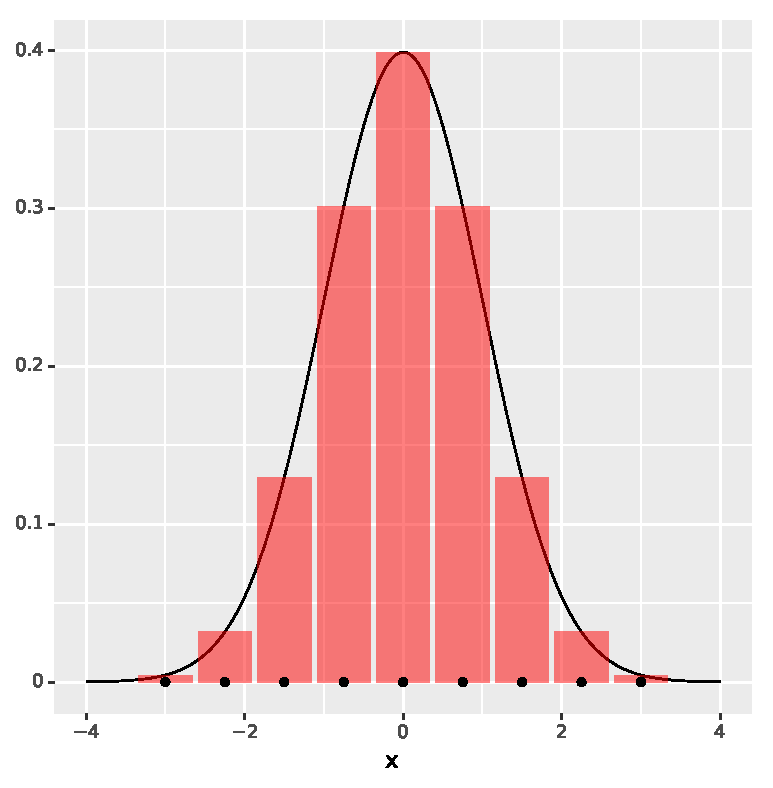
\includegraphics[scale=0.5]{1d_source_distribution}\hspace*{1cm}
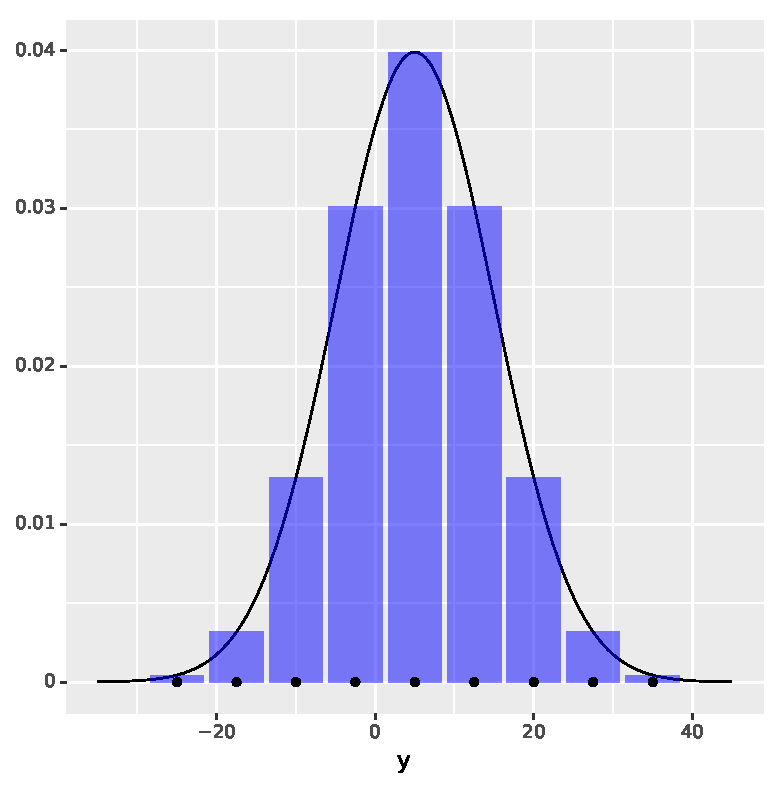
\includegraphics[scale=0.5]{1d_target_distribution}}

Let $y=ax + b$ the the relation between densities 
\begin{align*}
p_x(x)=\sigma\cdot p_y(y)
\end{align*}
follows form the fact that areas of red and blue columns must be the same.


\middlefoil{Motivating examples\vspace*{1ex}\\ {\large Supervised learning}}

\foilhead[-1cm]{Repeated experiments with external controls}

\illustration[scale=1.25]{general-model}

\textbf{Linear regression models}
\begin{triangles}
\item We assume that $y_i$ depends only on the values of $x_{i1}, \ldots, x_{i\ell}$ 
\item A linear model assumes $y_{i}=w_{1}x_{i1}+\cdots+ w_\ell x_{i\ell}+ w_{0}+\varepsilon_i$.
\item All error terms $\varepsilon_i$ are assumed to be independent.
\item  All error terms $\varepsilon_i$ are drawn from a normal distribution $\mathcal{N}(0,\sigma)$.
\end{triangles}




\foilhead[-1cm]{Higher-order Markov chains}
\illustration[scale=1.25]{markov-chain}

\textbf{Time-series models}
\begin{triangles}
\item We assume that $x_{i+1}$ depends only on the values of $x_i, \ldots, x_{i-\ell}$ 
\item A linear model assumes $x_{i+1}=w_0+w_{1}x_i+\cdots+ w_{\ell+1} x_{i-\ell}+\varepsilon_i$.
\item All error terms $\varepsilon_i$ are assumed to be independent.
\item  All error terms $\varepsilon_i$ are drawn from a normal distribution $\mathcal{N}(0,\sigma)$.
\end{triangles}





\foilhead[-1cm]{Univariate linear regression}

\begin{triangles}
\item Fix a set of inputs $x_1, \ldots, x_n\in \RR$. 
\item A probabilistic model is defined by three coefficients $a, b,\sigma\in\RR$.
\item The model assigns a probability to outcomes $y_1,\ldots, y_n$ through the following observation generation mechanism
\begin{align*}
  y_i=ax_i+b+\varepsilon_i,\qquad \varepsilon_i\sim\NNN(0,\sigma)
\end{align*}
\item Consequently 
\begin{align*}
  p[\vec{y}|\vec{x},a,b]&=\prod_{i=1}^n\frac{1}{\sqrt{2\pi}
    \sigma}\cdot\exp{-\frac{(y_i-ax_i-b)^2}{2\sigma^2}}
\end{align*}
\end{triangles}

\foilhead[-1cm]{Maximum likelihood estimate}

As usual we can find  $a,b,\sigma\in\RR$ that maximise the log-likelihood
\begin{align*}
\log p[\vec{y}|\vec{x},a,b,\sigma]&= const -n\log \sigma-\sum_{i=1}^n\frac{(y_i-ax_i-b)^2}{2\sigma^2}
\end{align*}
and thus we can find $a$ and $b$ by minimising 
\begin{align*}
\text{MSE}=\frac{1}{n}\cdot \sum_{i=1}^n(y_i-ax_i-b)^2\enspace.
\end{align*}


\foilhead[-1cm]{Residuals and the variance parameter}

For fixed $a, b\in\RR$ we can define predictions and residuals 
\begin{align*}
\hat{y}_i&= ax_i-b\\
r_i&=y_i-\hat{y}_i
\end{align*}
To find the optimal variance $\sigma^2$ we need to maximise
\begin{align*}
\log p[\vec{y}|\vec{x},a,b,\sigma]&= const -n\log \sigma-\sum_{i=1}^n\frac{r_i^2}{2\sigma^2}
\end{align*}
The resulting solution is 
\begin{align*}
\sigma^2=\frac{1}{n}\cdot \sum_{i=1}^n (y_i-\hat{y}_i)^2
\end{align*}



\foilhead[-1cm]{Linear time-series model}

\begin{triangles}
\item Fix a set of initial inputs $x_{-\ell}, \ldots, x_{0}\in \RR$. Denote them by $\vec{x}_\circ$. 
\item Think of $x_{1},x_{2},\ldots, x_n$ as observations. Denote them by $\vec{x}$.  
\item A probabilistic model for state transitions is defined as follows
\begin{align*}
  x_{i+1}=\underbrace{w_0 +w_1x_i+\ldots w_{\ell+1} x_{i-\ell}}_{\hat{x}_{i+1}}+\varepsilon_i,\qquad \varepsilon_i\sim\NNN(0,\sigma)
\end{align*}
\item Consequently 
\begin{align*}
 p[\vec{x}|\vec{x}_\circ,\vec{w},\sigma]&=\prod_{i=1}^n\frac{1}{\sqrt{2\pi}
    \sigma}\cdot\exp{-\frac{(x_i-\hat{x}_i)^2}{2\sigma^2}}
\end{align*}
\end{triangles}


 \foilhead[-1cm]{Maximum likelihood estimate}

As usual we can find  $\vec{w}\in \RR^{\ell+2}$ and $\sigma\in\RR$ that maximise the log-likelihood
\begin{align*}
\log p[\vec{x}|\vec{x}_\circ,\vec{\beta},\sigma]&= const -n\log \sigma-\sum_{i=1}^n\frac{(x_i-\hat{x}_i)^2}{2\sigma^2}
\end{align*}
and thus we can find $\vec{w}$ by minimising 
\begin{align*}
\text{MSE}=\frac{1}{n}\cdot \sum_{i=1}^n(x_i-w_0-w_1x_{i-1}-\ldots- w_{\ell+1} x_{i-1-\ell})^2\enspace.
\end{align*}

The latter is the standard multivariate linear regression setup. The variance of the model $\sigma^2$ can be found by the same formula as for linear regression.
 

\foilhead[-1cm]{Input values and numerical stability}

\begin{center}
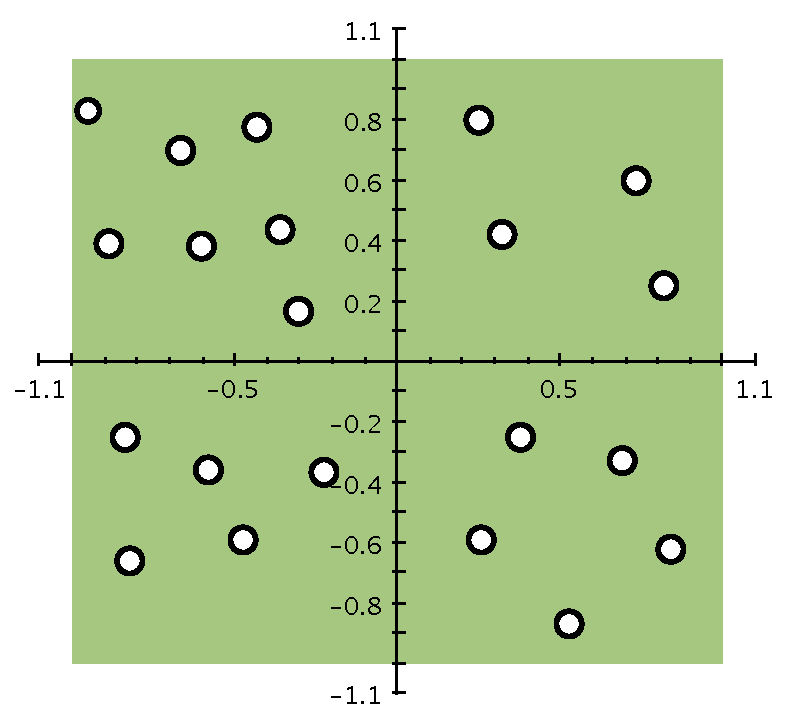
\includegraphics[scale=0.655]{good-layout}\hspace*{1cm}
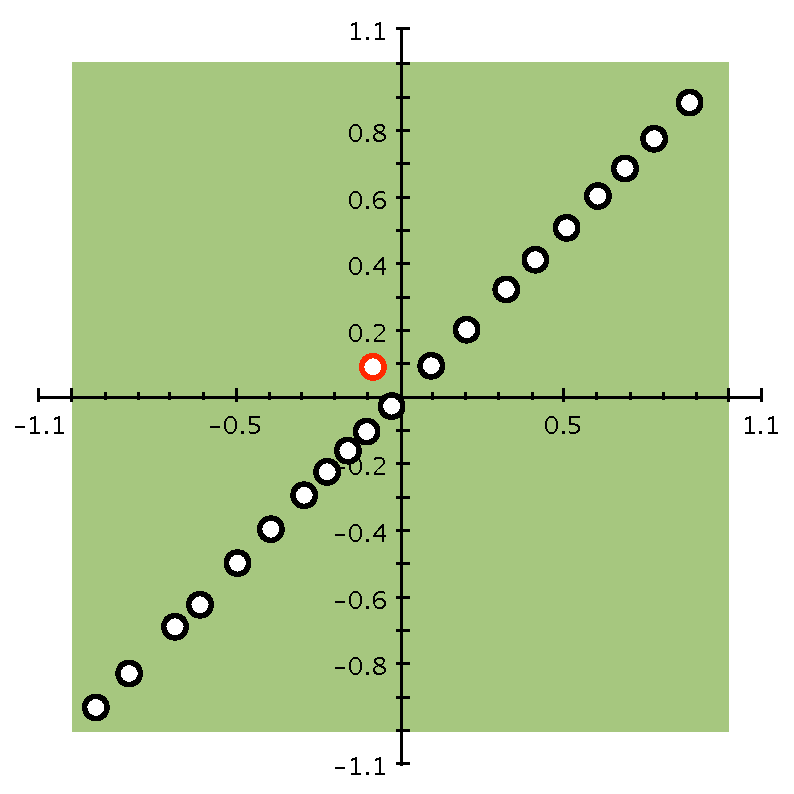
\includegraphics[scale=0.6]{bad-layout}
\end{center}

A small error in a point with big leverage can make linear regression function arbitrary large, which can lead to large test errors.
\begin{triangles}
\item In many case we know that the final output must be in fixed range.
\end{triangles}


\foilhead[-1cm]{Ridge regression}
%\enlargethispage{1cm}
Let us seek the prediction as a function $f(\vec{x})=w_1x_1+\cdots+w_kx_k$ with restriction $f(\vec{x})\leq c$ inside a unit ball $\norm{\vec{x}}_2^2=x_1^2+x_2^2+\cdots+x_k^2\leq 1$. 

\centerline{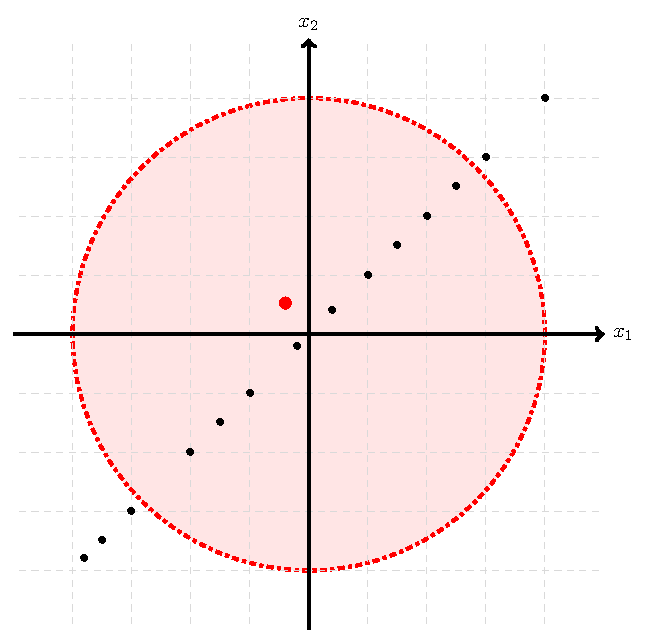
\includegraphics[scale=0.55]{ridge-constraint}}
\vspace*{-2ex}


Then we should solve the following task instead: \vspace*{-1.5ex}
\begin{align*}
&\frac{1}{N}\cdot\sum_{i=1}^N\bigl(y_i-f(\vec{x}_i)\bigr)^2\to \min\\
&\text{s.t. } w_1^2+\cdots+ w_k^2\leq c^2
\end{align*}




\foilhead[-1cm]{LASSO regression}

\enlargethispage{1cm}
Let us seek the prediction as a function $f(\vec{x})=w_1x_1+\cdots+w_kx_k$ with restriction $f(\vec{x})\leq c$ inside a unit ball $\norm{\vec{x}}_\infty=\max\set{\abs{x_1},\ldots,\abs{x_k}}\leq 1$. 

\centerline{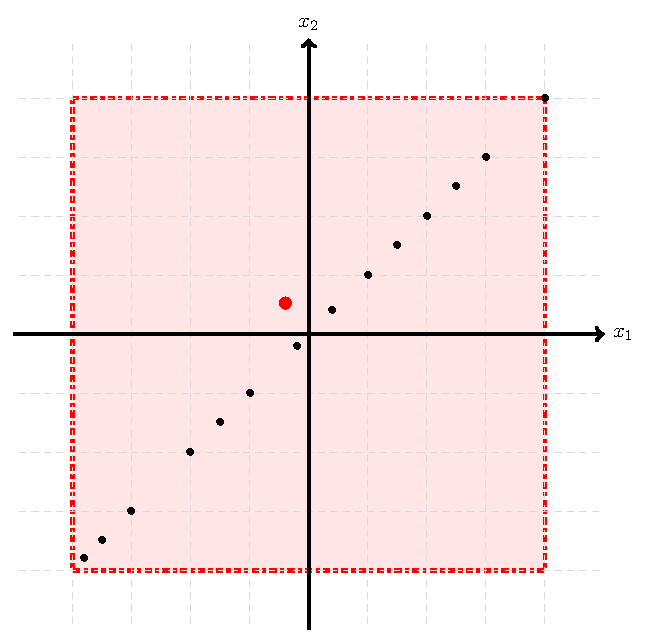
\includegraphics[scale=0.55]{lasso-constraint}}
\vspace*{-2ex}


Then we should solve the following task instead: \vspace*{-1.5ex}
\begin{align*}
&\frac{1}{N}\cdot\sum_{i=1}^N(y_i-f(\vec{x}_i))^2\to \min\\
&\text{s.t. } \abs{w_1}+\cdots+\abs{w_k}\leq c
\end{align*}



\foilhead[-1cm]{Lagrange' trick}


If we want to  minimise $f(\vec{x})$ such that $g(\vec{x})\leq c$ for a non-negative function $g(\cdot)$, then there exists             $\lambda\geq 0$ such that the solution of the original problem is a minimum for a modified function
\begin{align*}
f_*(\vec{x})=f(\vec{x}) + \lambda g(\vec{x})
\end{align*}

\textbf{Consequences}
\begin{triangles}
\item  We can use  a penalty term $\lambda \norm{\vec{w}}_1$ for rectangular area
\item We can use  a penalty term $\lambda \norm{\vec{w}}_2^2$ for circular area
\end{triangles}



\middlefoil{Multivariate normal\vspace*{2ex}\\ distribution}


\foilhead[-1cm]{White Gaussian noise}

\illustration[scale=0.4]{white_gaussian_noise}
\vspace*{-1.0cm}

\textbf{Definition.} A random vector $X_1,\ldots, X_n$ is a standard normal random vector if all of its components are independent and and $X_i\sim \NNN(0,1)$.
\begin{triangles}
\item The density can be computed based on independence:
\begin{align*}
p(x_1,\ldots,x_n)=p(x_1)\cdots p(x_n)=\frac{1}{(2\pi)^{n/2}}\cdot\mathsf{exp}\Biggl(-\frac{x_1^2+\cdots+x_n^2}{2}\Biggl)\enspace.
\end{align*}
\end{triangles}

\foilhead[-1cm]{Scaling and shifting}

By shifting and scaling the source distribution $\NNN(\vec{0},I)$ we can obtain some other instances of multivariate normal distribution.
\vspace*{-1cm}

\begin{center}
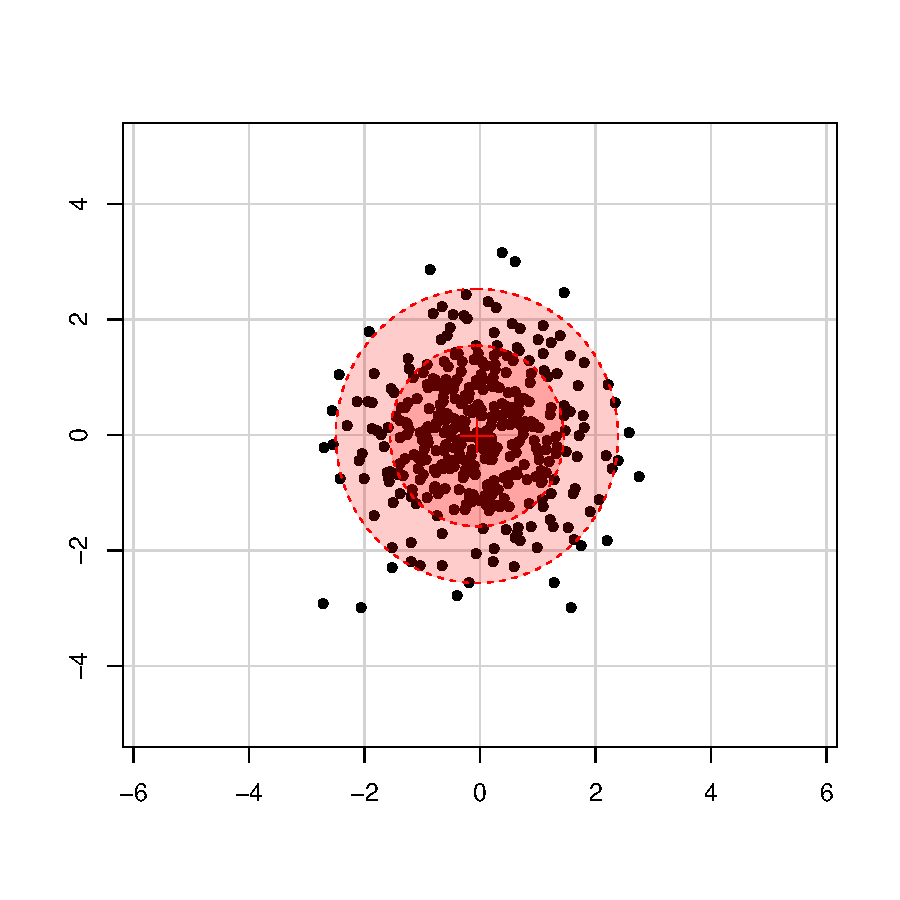
\includegraphics[scale=0.65]{source-distribution.pdf}
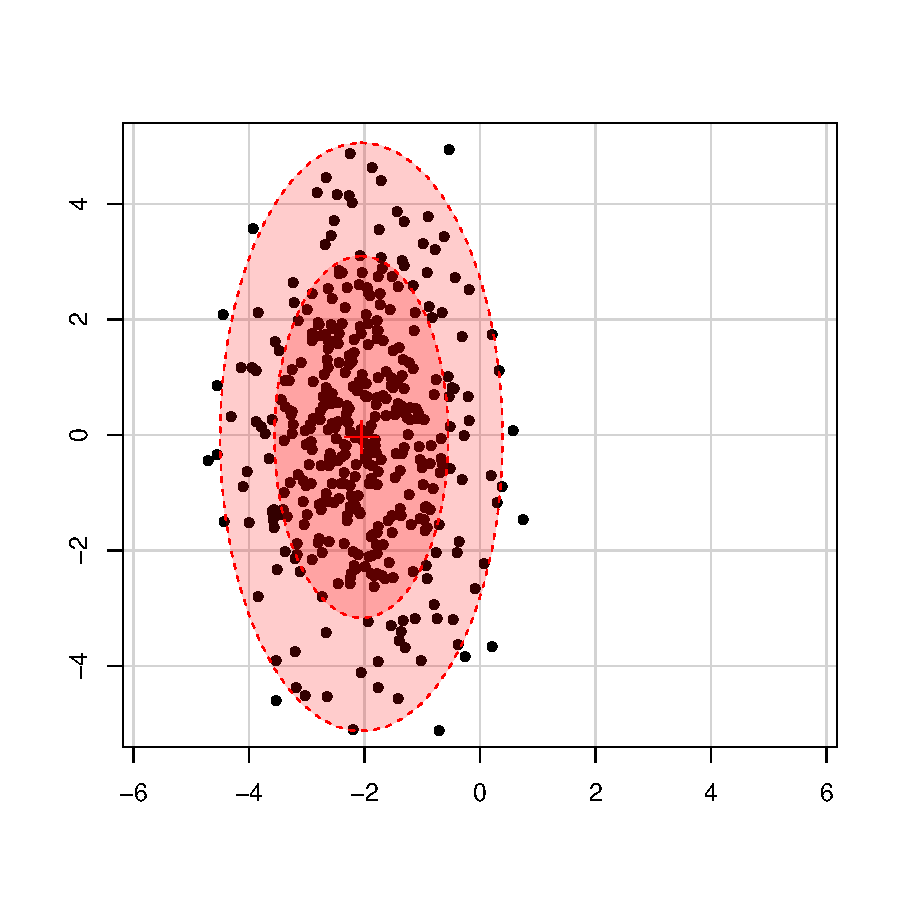
\includegraphics[scale=0.65]{scaled-distribution.pdf}
\end{center}\vspace*{-10cm}





\foilhead[-1cm]{Necessity of rotations}

As the choice of coordinate axis is sometimes arbitrary, there must be other ways to form a normal distribution -- rotations of coordinate axis.\vspace*{-1cm}  

\begin{center}
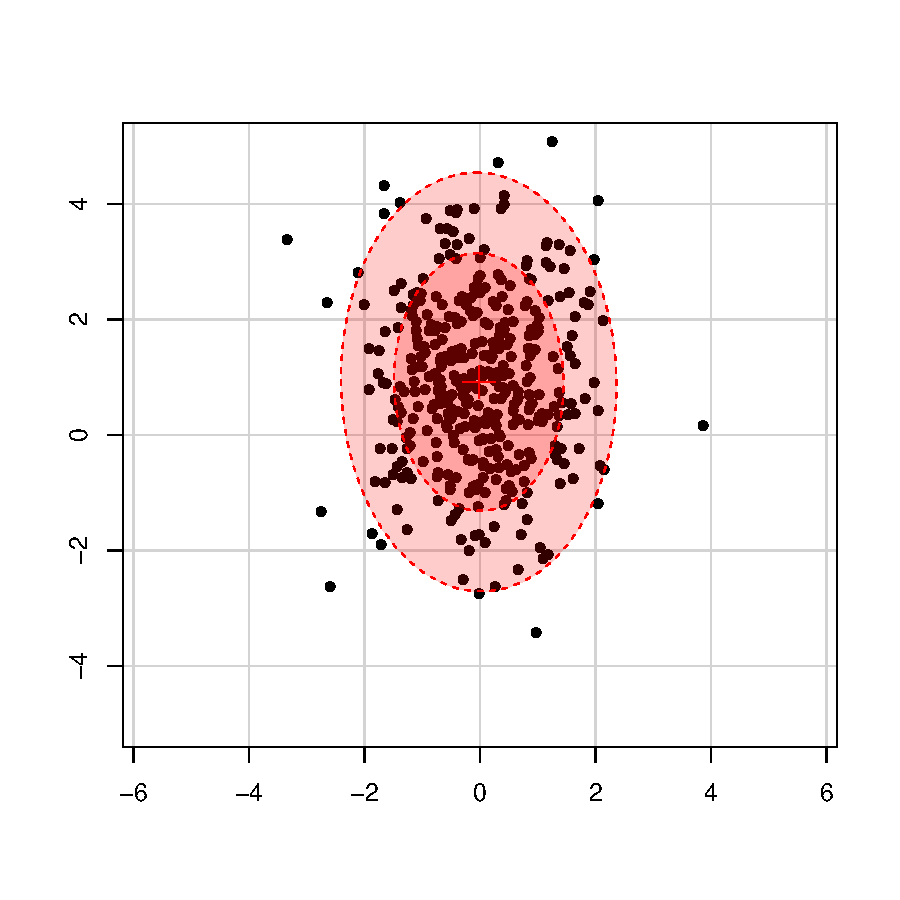
\includegraphics[scale=0.65]{two-dimensional-normal-distribution-i.pdf}
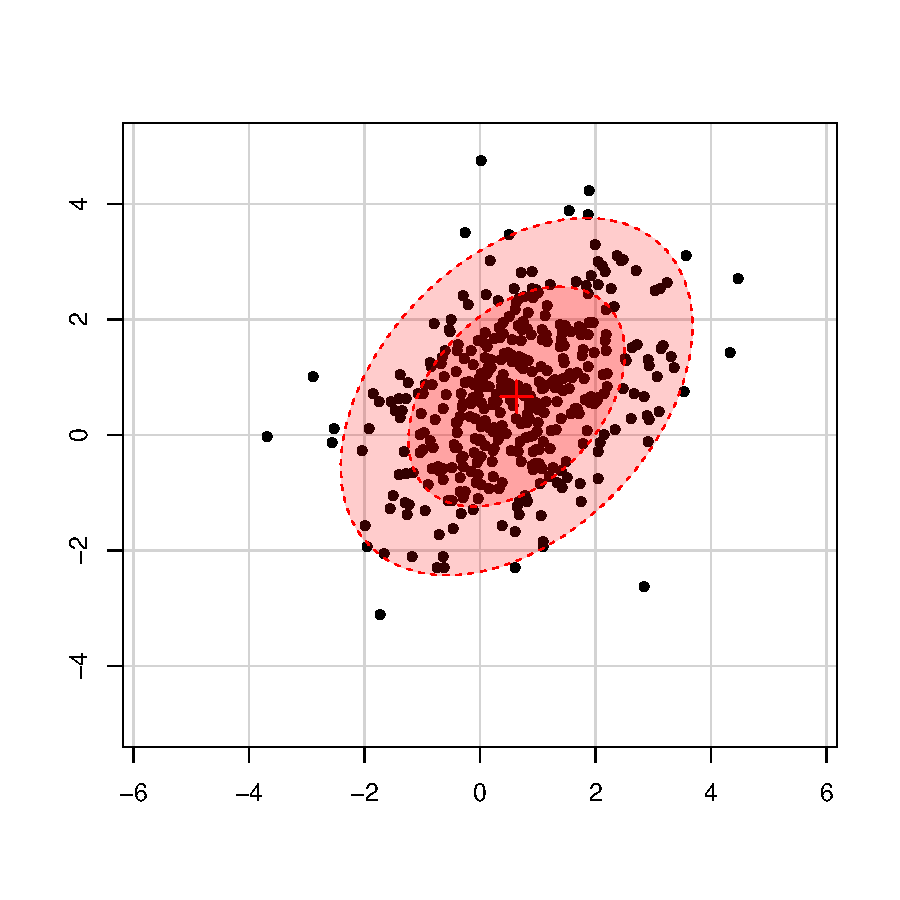
\includegraphics[scale=0.65]{two-dimensional-normal-distribution-ii.pdf}
\end{center}\vspace*{-1cm}

Any affine transformation can be expressed as scaling, rotating and shifting.




\foilhead[-1cm]{Affine transformations}

Let $\vec{x}$ be standard normal random vector and let $\vec{y}$ be obtained the scaling,  translation and rotation of the coordinate plane.

Then we can express $\vec{x}$ and $\vec{y}$ in terms of an affine transformation
\begin{align*}
  \vec{y}&=A\vec{x}+\vec{\mu} \enspace,\\
  \vec{x}&=A^{-1}(\vec{y}-\vec{\mu}) \enspace.
\end{align*}

\textbf{Observation.}
Affine transformations are closed with respect to composition, i.e., applying two affine transformations yields a new affine transformation. \vspace*{2ex}

\textbf{Remark.} Not all affine transformations are invertible.\lastline


\foilhead[-1cm]{What is density in 2D?}


Recall that density assigns probability to small enough regions $\RRR$:
\begin{align*}
\Pr_{x_1^*,x_2^*}
\left[\begin{aligned}
   &x_1\leq x_1^*\leq x_1+\Delta x_1\\ 
   &x_2\leq x_2^*\leq x_2+\Delta x_2
\end{aligned}\right]= p(x_1,x_2)\cdot\underbrace{\Delta x_1\Delta x_2}_S +\, \varepsilon
\end{align*}
where $\varepsilon=o(\Delta x_1\cdot\Delta x_2)$ in the process $\Delta x_1\to 0$ and $\Delta x_2\to 0$.\vspace*{1cm}

\textbf{Remark.} Regions $\RRR$ do not have to be rectangular as long as:
\begin{triangles}
\item The area $S(\RRR)$ of a region can be computed.  
\item Probability can be assigned to the region $\RRR$ and its scalings.
\end{triangles}
Then $\varepsilon=o(S)$ when we rescale the region $\RRR$ around the point $(x_1,x_2)$.


\foilhead[-1cm]{Density recalibration}

Any affine transformation changes a square grid into parallelograms. \vspace*{-1cm}
\begin{center}
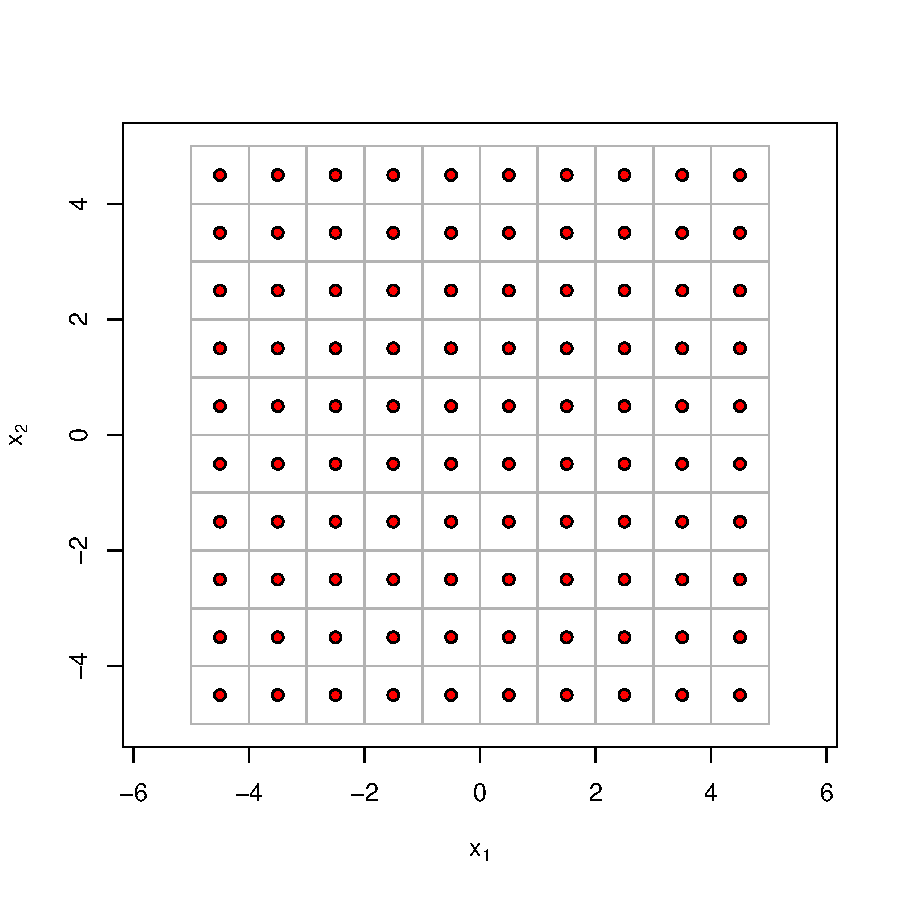
\includegraphics[scale=0.55]{original-grid.pdf}
\raisebox{4.0cm}{$\quad\xrightarrow{\vec{y}=A\vec{x}+\vec{\mu}}\quad$}
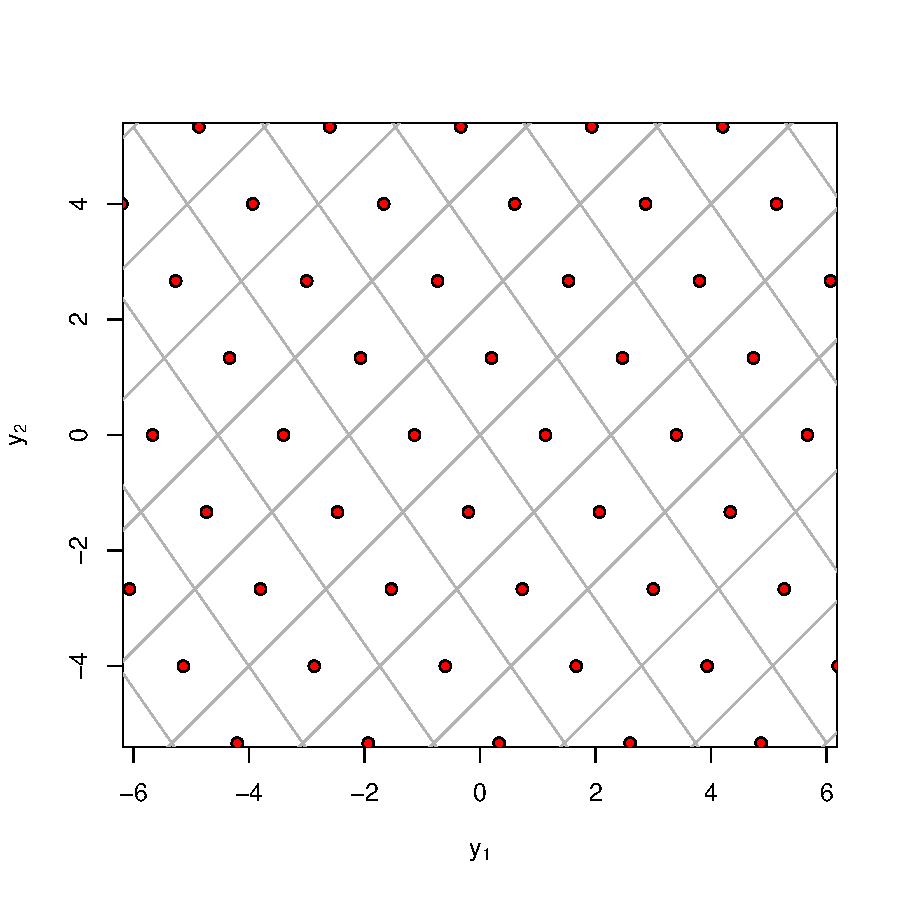
\includegraphics[scale=0.55]{transformed-grid.pdf}
\end{center}\vspace*{-1cm}

As a result, the area of the regions is different on the left and on the right:
\begin{align*}
p(x_1,x_2)\cdot S_1\approx q(y_1,y_2)\cdot S_2\qquad\Longrightarrow\qquad q(y_1,y_2)={\frac{S_1}{S_2}}\cdot p(x_1,x_2) 
\end{align*}
Fortunately, the ratio between areas are constant over the entire plane!\lastline

  
\foilhead[-1cm]{Density of two-variate normal distribution}

\enlargethispage{1cm}
The density of $(x_1,x_2)$ pairs can be computed based on independence:
\begin{align*}
p(x_1,x_2)=p(x_1)\cdot p(x_2)=\frac{1}{2\pi}\cdot\mathsf{exp}\Biggl(-\frac{x_1^2+x_2^2}{2}\Biggl)\enspace.
\end{align*}
\vspace*{-3ex}

To estimate density $q(y_1,y_2)$, we must find the corresponding $(x_1,x_2)$:
\begin{align*}
 \vec{y}=A\vec{x}+\vec{\mu}\quad\Leftrightarrow\quad \vec{x}=A^{-1}(\vec{y}-\vec{\mu})\enspace. 
\end{align*}
Thus we get \vspace*{-2ex}
\begin{align*}
q(y_1,y_2)&=\frac{S_1}{S_2}\cdot\frac{1}{2\pi}\cdot
\exp{-\frac{(\vec{y}-\vec{\mu})^T A^{-T}A^{-1}(\vec{y}-\vec{\mu})}{2}}\\
&=\frac{1}{\sqrt{\det(\Sigma)}}\cdot\frac{1}{2\pi}\cdot
\exp{-\frac{(\vec{y}-\vec{\mu})^T \Sigma^{-1}(\vec{y}-\vec{\mu})}{2}}\enspace.
\end{align*}

 

\foilhead[-1cm]{Illustrative example}
 
\begin{center}
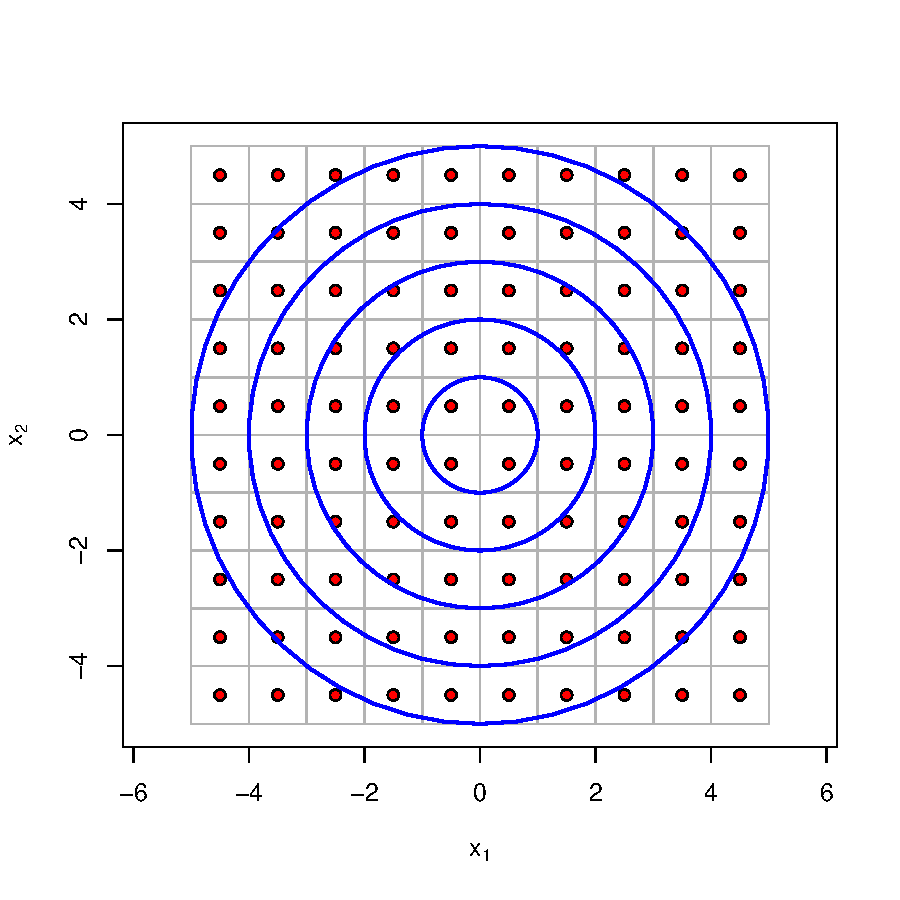
\includegraphics[scale=0.55]{original-contours.pdf}
\raisebox{4.0cm}{$\quad\xrightarrow{\vec{y}=A\vec{x}+\vec{\mu}}\quad$}
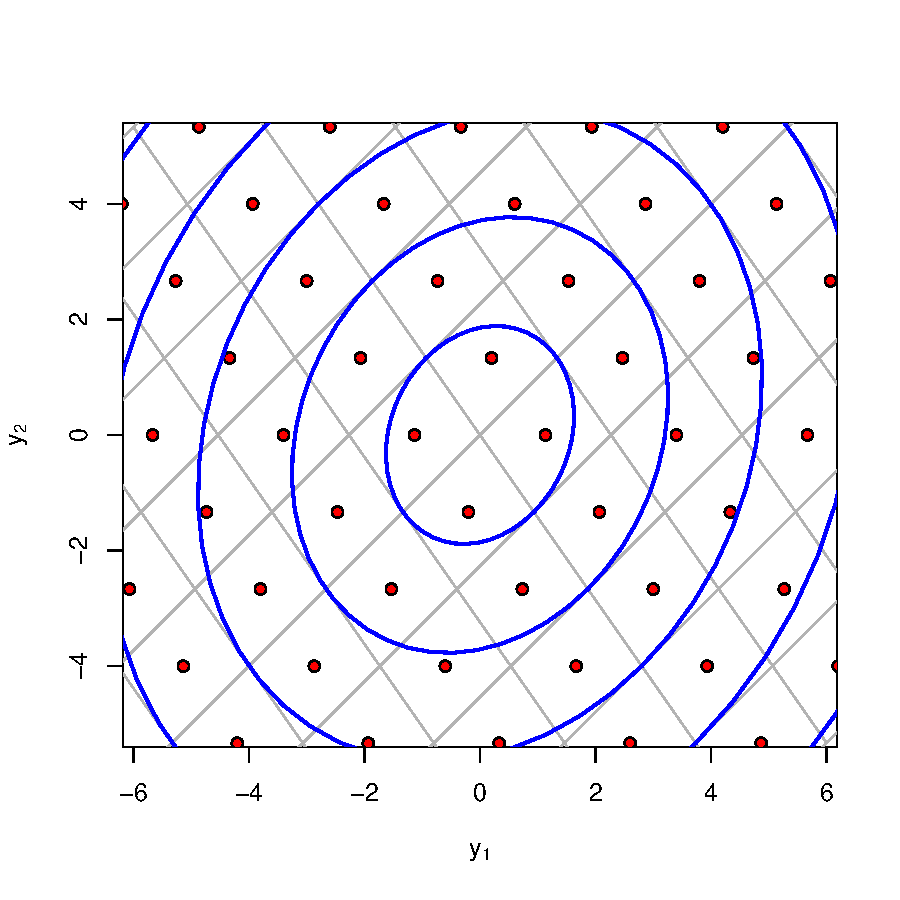
\includegraphics[scale=0.55]{transformed-contours.pdf}
\end{center}\vspace*{-0cm}

\begin{triangles}
\item Affine transformation changes the square grid into parallelograms. 
\item Affine transformation changes circular equiprobability lines into ellipses. 
\item The axes of the ellipses may intersect with the sides of parallelograms.
\end{triangles}



\foilhead[-1cm]{Generalisation to multivariate case}

If observed quantities $\vec{y}$ are generated by applying the affine transformation 
\begin{align*}
 \vec{y}=A\vec{x}+\vec{\mu}\quad\Leftrightarrow\quad \vec{x}=A^{-1}(\vec{y}-\vec{\mu})\enspace
\end{align*}
to the \emph{independent source signals} $x_1,\ldots, x_n\sim\NNN(0,1)$, then the resulting distribution is \emph{a multivariate normal distribution} with the density:
\begin{align*}
p(\vec{y})&=\frac{1}{(2\pi)^{n/2}}\cdot\frac{1}{\sqrt{\det(\Sigma)}}\cdot
\exp{-\frac{(\vec{y}-\vec{\mu})^T \Sigma^{-1}(\vec{y}-\vec{\mu})}{2}}\enspace
\end{align*} 
where $\Sigma^{-1}=A^{-T}A^{-1}$ is \emph{a positively definite symmetric matrix}.



\middlefoil{Important properties of\vspace*{1ex}\\ normal distributions}

\foilhead[-1cm]{Closeness under marginalisation}

Let $\vec{x}_{\III}=(x_i)_{i\in\III}$ be a subvector determined by the coordinate set $\III$.
Then $\vec{x}_{\III}$ is distributed according to a multivariate normal distribution as long as 
the vector $\vec{x}$ comes form a multivariate normal distribution $\NNN(\vec{\mu},\Sigma)$.

\begin{triangles}
\item Moment matching gives the parameters of the resulting distribution 
\begin{align*}
\EXP(\vec{x}_{\III})&= \EXP(\vec{x})_{\III}=\vec{\mu}_{\III} \\
\COV(\vec{x}_{\III})&=\COV(\vec{x})_{\III\times \III}=\Sigma[\III, \III]
\end{align*}
\end{triangles}

\foilhead[-1cm]{Closeness under linear combinations}

Linear combination $y=\vec{\alpha}_1^T \vec{x}_1+\vec{\alpha}_2^T\vec{x}_2$ of independent multivariate normal distributions $\vec{x}_1\sim\NNN(\vec{\mu}_1,\Sigma_1)$ and $\vec{x}_2\sim\NNN(\vec{\mu}_2,\Sigma_2)$ is also  a multivariate normal distribution.

\begin{triangles}
\item Moment matching gives the parameters of the resulting distribution 
\begin{align*}
\EXP(y)&= \vec{\alpha}_1^T\EXP(\vec{x}_1)+\vec{\alpha}_2^T\EXP(\vec{x}_2)=
\vec{\alpha}_1^T\vec{\mu}_1+\vec{\alpha}_2^T\vec{\mu}_2\\
\VAR(y)&=\COV(\vec{\alpha}_1^T \vec{x}_1) + \COV(\vec{\alpha}_2^T \vec{x}_2)\\
&=\vec{\alpha}_1^T \COV(\vec{x}_1)\vec{\alpha}_1+ \vec{\alpha}_2^T \COV(\vec{x}_2)\vec{\alpha}_2\\
&=\vec{\alpha}_1^T \Sigma_1\vec{\alpha}_1+ \vec{\alpha}_2^T \Sigma_2\vec{\alpha}_2
\end{align*}
\item Closeness under linear combinations holds also for matrix combinations. 
\end{triangles}

\foilhead[-1cm]{Closeness under conditioning}

Let $\vec{x}$ and $\vec{y}$ be related random variables. 
Let $\vec{x}|\vec{y}_*$ denote the conditional distribution of $\vec{x}$ given that a random variable $\vec{y}$ has a fixed value $\vec{y}_*$.
Then $\vec{x}|\vec{y}_*$ is distributed according to a multivariate normal distribution provided that 
 $(\vec{x},\vec{y})$ comes form a multivariate normal distribution $\NNN((\vec{\mu}_i),(\Sigma_{ij}))$

\begin{triangles}
\item Moment matching gives the parameters of the resulting distribution 
\begin{align*}
\EXP(\vec{x}|\vec{y}_*)&= \vec{\mu}_1+ \Sigma_{1,2}\Sigma_{2,2}^{-1}(\vec{y}-\vec{\mu}_2)\\
\COV(\vec{x}|\vec{y}_*)&= \Sigma_{1,1}-\Sigma_{1,2}\Sigma_{2,2}^{-1}\Sigma_{2,1}\\
\end{align*}
\end{triangles}


\middlefoil{Motivating examples\vspace*{1ex}\\ {\large Filtering and smoothing}}

\foilhead[-1cm]{Prediction of vector values}


Prediction errors of different vector components can be correlated.
\vspace*{3ex} 

\illustration[scale=0.5]{colored-residuals}

As a result combined model can outperform coordinatewise predictions. \vspace*{-2ex}

\foilhead[-1cm]{Prediction intervals for time-series}

\illustration{markov-chain}

After we have fitted the linear regrssion model to timeseries data we might want to compute prediction intervals for iterative stepwise predictions.

\begin{triangles}
\item Let $\vec{x}_0$ be the known initial state and $\vec{x}_1, \ldots, \vec{x}_n$ iterative predictions.
\item We need priors $\pi[\vec{x}_i]=p[\vec{x}_i|\vec{x}_0]$ to compute confidence intervals.
\item It turns out that all priors $p[\vec{x}_i]$ are normal distributions.
\item Moment matching allows us to learn the parameters of the distributions.
\end{triangles}


\foilhead[-1cm]{Smoothing and reverse Markov chain}

\illustration{reverse-markov-chain}

Sometimes we have to interpolate observations in the time series. This can be stated as amoothing task where we know $\vec{x}_0$ and $\vec{x}_n$.

\begin{triangles}
\item We need likelihoods $\lambda[\vec{x}_i]=p[\vec{x}_n|\vec{x}_i]$ for the smoothing.
\item Likelihood propagation formula is analogous to the prior propagation.
\item We can define a reverse Markov chain such that the prior $\pi^*[\vec{x}_i]\propto \lambda[\vec{x}_i]$. 
\item The resulting chain has reversed dynamics. 
\item It turns out that all likelihoods $\lambda[\vec{x}_i]$ are normal distributions.
\item The posterior as product $\pi[\vec{x}_i]\cdot \lambda[\vec{x}_i]$ is also a normal distribution.
\end{triangles}


\foilhead[-1cm]{Sensor fusion with Hidden Markov Models}


\illustration[scale=1.0]{continuous-hidden-markov-model}

A standard problem in robotics or machine perception is following.
\begin{triangles}
\item Several sensors measure a physical system
\item Measurements are observable as $\vec{y}\in\RR^p$.
\item Physical system has an hidden state $\vec{x}\in\RR^n$.
\item Physical system evolves linearly $\vec{x}_{i+1}=A\vec{x}_i+\vec{w}_i$.
\item Measurements are linear from the state $\vec{y}_{i}=C\vec{x}_i+\vec{v}_i$.
\item Distribution of error terms $\vec{v}_i$ and $\vec{w}_i$ is known.  
\item Error terms $\vec{v}_i$ and $\vec{w}_i$ are independently drawn.
\end{triangles}

\foilhead[-1cm]{Kalman filter}

\illustration[scale=1.0]{kalman-filter}

As before we can consider the prior and filter densities
\begin{align*}
\pi[\vec{x}_i]&=p[\vec{x}_i|\vec{y}_1,\ldots, \vec{y}_{i-1}]\\
f[\vec{x}_i]&=p[\vec{x}_i|\vec{y}_1,\ldots, \vec{y}_{i}]\propto \pi[\vec{x}_i]\cdot p[\vec{y}_i|\vec{x}_i]
\end{align*}
A similar update logic assures that both distributions are normal distributions and that we can only compute the parameters of these normal distributions. 
 
\foilhead[-1cm]{Smoothing and reverse Hidden Markov Model}

\illustration[scale=1.0]{reverse-hidden-markov-model}

\begin{triangles}
\item We need likelihoods $\lambda[\vec{x}_i]=p[\vec{y}_{i+1},\ldots, \vec{y_n}|\vec{x}_i]$ for the smoothing.
\item Likelihood propagation formula is analogous to the prior propagation.
\item We can define a reverse HMM such that the prior $\pi^*[\vec{x}_i]\propto \lambda[\vec{x}_i]$.
\item The resulting HMM has reversed dynamics. 
\item It turns out that all likelihoods $\lambda[\vec{x}_i]$ are normal distributions.
\item The posterior as product $\pi[\vec{x}_i]\cdot \lambda[\vec{x}_i]\cdot p[\vec{y}_i|\vec{x}_i]$ is also a normal distribution.
\end{triangles}


\middlefoil{Motivating examples\vspace*{1ex}\\ {\large Markov fields}}




\foilhead[-1cm]{Background model for digital images}
\illustration[scale=0.8]{markov-random-field-i}

In most images intensity of pixel is influenced only by its neighbours:
\begin{triangles}
\item For simple textures the neighbourhood consist of four adjacent pixels.
\item For complex textures the the neighbourhood contains much more pixels.
\item For homogenous textures the conditional probabilities are universal\vspace*{0.5ex}.
\begin{diamonds}
\item Generative repetitive patterns for textile and grass\vspace*{1ex}   
\end{diamonds}

\item For complex patterns conditional probabilities can be location dependent.\vspace*{0.5ex}

\begin{diamonds}
\item Generative patterns for human faces and fashion accessories 
\end{diamonds}
\end{triangles}

\foilhead[-1cm]{Random Markov Fields}

\illustration[scale=1.2]{markov-random-field}

\textbf{Definition.}
Markov random field is specified by undirected graph connecting random variables $X_1,X_2,\ldots$ such that for any node $X_i$ 
\begin{align*}
\pr{x_i|(x_j)_{j\neq i}}=\pr{x_i| (x_j)_{j\in\NNN(X_i)} }
\end{align*}
where the set of neighbours $\NNN(X_i)$ is also known as \emph{Markov blanket} for $X_i$. 


\foilhead[-1cm]{Hammersley-Clifford theorem}

The probability of an observation $\vec{x}=(x_1,x_2,\ldots)$ generated by a Markov random field can be expressed in the form 
\begin{align*}
\pr{\vec{x}}=\frac{1}{Z(\omega)}\cdot\exp{-\sum_{c\in\textsf{MaxClique}}\Psi_c(\vec{x}_c,\omega)} 
\end{align*}  
where
\begin{triangles}
\item $Z(\omega)$ is a normalising constant
\item $\textsf{MaxClique}$ is the set of maximal cliques in the Markov random field
\item $\Psi_c$ is defined on the variables in the clique $c$ 
\end{triangles}
\vspace*{2ex}

The formula implies that the distribution belongs to the exponential family.

\begin{triangles}
\item Multivariate normal distribution belongs to the exponential family
\end{triangles}


\foilhead[-1cm]{Conditional Random Fields}

\illustration[scale=1.5]{conditional-random-field}

\textbf{Definition.}
Let $X_1,X_2,\ldots$ and $Y_1,Y_2,\ldots$ be random variables. The entire process is conditional random field if random variables $Y_1,Y_2,\ldots$ conditioned for any sequence of observations $x_1,x_2,\ldots$ form a Markov random field
\begin{align*}
\pr{y_i|(x_k)_{k=1}^\infty, (y_j)_{j\neq i}}=\pr{y_i|(x_k)_{k=1}^\infty, (y_j)_{j\in\NNN(Y_i)} }
\end{align*}
where the set of neighbours $\NNN(Y_i)$ is a \emph{conditional Markov blanket} for $Y_i$. 



\foilhead[-1cm]{Image segmentation and sequence labelling}
\enlargethispage{1cm}
\illustration[scale=1.0]{conditional-random-field}


\begin{triangles}
\item The input $\vec{x}$ is used to predict labels $y_1,y_2,\ldots$.
\item A correct label sequence must satisfy possibly unknown restrictions.
\item These restrictions are captured by conditional random random field.
\end{triangles}\vspace*{0.5cm}


\textbf{Consequences of Hammersley-Clifford theorem}
\begin{triangles}
\item Clique features $\Psi_c$ can depend on $(y_i)_{i\in c}$, $(x_i)_{i=1}^\infty$ 
\item Features can be defined as linear combination of vertex and edge features.
\item A vertex feature looks only variable $y_i$ associated with the vertex.
\item An edge feature looks only variables $y_i, y_j$ associated with the edge.
\end{triangles}





\middlefoil{Markov fields\vspace*{0ex}\\ with\vspace*{1ex}\\ multivariate normal distributions}



\foilhead[-1cm]{General form of the likelihood function}

The celebrated Hammersley-Clifford theorem fixes the format in which the corresponding probability distribution must be sought:
\begin{align*}
p[\vec{x}|\omega]=\frac{1}{Z(\omega)}\cdot\exp{-\sum_{c\in\textsf{MaxClique}}\Psi_c(\vec{x}_c,\omega)} 
\end{align*} 
where 
\begin{triangles}
\item $\omega$ is a set of model parameters
\item $Z(\omega)$ is a normalising constant
\item $\textsf{MaxClique}$ is the set of maximal cliques in the Markov random field
\item $\Psi_c$ is defined on the variables $x_i$ in the clique $c$. 
\end{triangles}

\foilhead[-1cm]{Multivariate normal distribution as likelihood}

If individual sub-potentials $\Psi_c(\vec{x}_c,\omega)$ are quadratic forms then the energy 
\begin{align*}
\Psi(\vec{x})=\sum_{c\in\textsf{MaxClique}}\Psi_c(\vec{x}_c,\omega) 
\end{align*} 
is also a quadratic form and thus $p[\vec{x}|\omega]$ is a multivariate normal distribution.\vspace*{1cm}

Sub-potentials are often fixed directly based on smoothness constraints
\begin{triangles}
\item Intensities have bounded variance: $\Psi_e=\delta^2 x_{ij}^2$. 
\item Intensity changes smoothly vertically: $\Psi_e=\beta(x_{i,j}-x_{i+1,j})^2$.
\item Intensity changes smoothly horizontally: $\Psi_e=\alpha(x_{i,j}-x_{i,j+1})^2$.
\end{triangles} 

\foilhead[-1cm]{Toy example}

\illustration[scale=1.0]{markov-random-field-iv}\vspace*{-0.6cm}

Sub-potentials corresponding four edges are:  
\begin{align*}
\Psi_1(x_1,x_2)&= \alpha_1(x_{1}-x_2)^2=\alpha_1 x_1^2-2\alpha_1 x_1x_2+\alpha_1 x_2^2\\
\Psi_2(x_2,x_3)&= \alpha_2(x_{2}-x_3)^2=\alpha_2 x_2^2-2\alpha_2 x_2x_3+\alpha_2 x_3^2\\
\Psi_3(x_3,x_4)&= \alpha_3(x_{3}-x_4)^2=\alpha_3 x_3^2-2\alpha_3 x_3x_4+\alpha_3 x_4^2\\
\Psi_4(x_4,x_1)&= \alpha_4(x_{4}-x_1)^2=\alpha_4 x_4^2-2\alpha_4 x_4x_1+\alpha_4 x_1^2
\end{align*}
Sub-potentials corresponding to four vertices are $\Psi_i^*(x_i)=\delta_i^2 x_i^2$ 

\foilhead[-1cm]{Resulting potential function}

\begin{align*}
\Psi(\vec{x})=\vec{x}^T
\begin{pmatrix}
\alpha_1+\alpha_4+\delta_1^2 & -\alpha_1 & 0 & -\alpha_4\\
-\alpha_1 &\alpha_1+\alpha_2+\delta_2^2 & -\alpha_2 & 0 \\
0 &-\alpha_2 &\alpha_2+\alpha_3+\delta_3^2 & -\alpha_3 \\
-\alpha_4 & 0 &-\alpha_3 &\alpha_3+\alpha_4+\delta_4^2 
\end{pmatrix}
\vec{x}
\end{align*}
and thus the covariance matrix $\Sigma$ and mean $\vec{\mu}$ can be computed by matching the shape of the multivariate normal density
\begin{align*}
p[\vec{x}|\vec{\mu},\Sigma]\propto\frac{1}{\sqrt{\det\Sigma}}\cdot\exp{-\frac{1}{2}\cdot 
(\vec{x}-\vec{\mu})^T\Sigma^{-1}(\vec{x}-\vec{\mu})}
\end{align*}





\end{document}
